\documentclass[11pt]{beamer}
\usetheme{Warsaw}
\usepackage[utf8]{inputenc}
\usepackage{amsmath}
\usepackage{amsfonts}
\usepackage{amssymb}
\usepackage{graphicx}
\setbeamersize{text margin left=6pt,text margin right=6pt}

\author{Agustín Curto}
\title{Turing vence a von Neumann}
\setbeamercovered{transparent}
\setbeamertemplate{navigation symbols}{}
\logo{}
\institute{FaMAF}
\date{2017}

\newcommand{\SIGMA}{\Sigma^{\ast}}
\newcommand{\PN}{\par\noindent}

\begin{document}

\begin{frame}
	\titlepage
\end{frame}

\begin{frame}
	\textbf{Notación}: dados $x_{1}, \dotsc, x_{n} \in \omega$ y $\alpha_{1}, \dotsc,\alpha_{m} \in \SIGMA$, con $n, m \in
	\omega $, usaremos:
	\begin{equation*}
		\lVert x_{1}, \dotsc, x_{n}, \alpha_{1}, \dotsc, \alpha_{m} \rVert
	\end{equation*}

	\PN para denotar el estado
	\begin{equation*}
		\left((x_{1}, \dotsc, x_{n}, 0, \dotsc), (\alpha_{1}, \dotsc, \alpha_{m}, \varepsilon, \dotsc)\right)
	\end{equation*}

	\PN Notese que por ejemplo:
	\begin{eqnarray*}
	\lVert x \rVert &=& \left((x, 0, \dotsc), (\varepsilon, \dotsc)\right) \text{Para } n = 1, m = 0 \\
	\lVert \Diamond \rVert &=& \left((0, \dotsc), (\varepsilon, \dotsc)\right) \text{Para } n = m = 0
	\end{eqnarray*}

	\PN Ademas es claro que:
	\[
		\lVert x_{1}, \dotsc, x_{n}, \alpha_{1}, \dotsc, \alpha_{m} \rVert = \lVert x_{1}, \dotsc, x_{n},
		\overset{i}{\overbrace{0, \dotsc, 0}}, \alpha_{1}, \dotsc, \alpha_{m}, \overset{j}{\overbrace{\varepsilon, \dotsc,
		\varepsilon}} \rVert
	\]
	cualesquiera sean $i, j \in \omega$.
\end{frame}

\begin{frame}
	\textbf{Probaremos}: Si $f$ es una función $\Sigma$-mixta que es computada por un programa $\mathcal{P} \in
	\mathrm{Pro}^{\Sigma}$, entonces existe una máquina de Turing deterministica con unit $M$ la cual computa a $f$.

	\vspace{3mm}
	\textbf{Definición}: Dado $\mathcal{P} \in \mathrm{Pro}^{\Sigma}$, definamos:
	\begin{eqnarray*}
		N(\mathcal{P}) &=& \mathrm{menor}\ k \in \mathbf{N}\ \mathrm{tal\ que\ las\ variables\ que\ ocurren\ en\ }
			\mathcal{P} \\
		&& \mathrm{esta} \text{n} \mathrm{\ todas\ en\ la\ lista\ N}1, \dotsc, \mathrm{N}\bar{k}, \mathrm{P}1, \dotsc,
			\mathrm{P}\bar{k}
	\end{eqnarray*}

	\PN \underline{Ejemplo}: Sea $\Sigma = \{\&,\#\}$, si $\mathcal{P}$ es el siguiente programa:
	\begin{equation*}
		\begin{array}{ll}
			\mathrm{L}1 & \mathrm{N}4\leftarrow \mathrm{N}4+1 \\
			& \mathrm{P}1\leftarrow \mathrm{P}1.\& \\
			& \mathrm{IF\ N}1\neq 0\ \mathrm{GOTO}\;\mathrm{L}1
		\end{array}
	\end{equation*}
	entonces tenemos $N(\mathcal{P})=4$
\end{frame}

\begin{frame}
	\PN Sea $\mathcal{P}$ un programa y sea $k$ fijo y $k \leq N(\mathcal{P})$. Describiremos como puede construirse una
	máquina de Turing la cual simulará a $\mathcal{P}$. La construcción de la máquina simuladora dependerá de
	$\mathcal{P}$ y de $k$.

	\PN Nótese que cuando $\mathcal{P}$ se corre desde algún estado de la forma
	\begin{equation*}
		\lVert x_{1}, \dotsc, x_{k}, \alpha_{1}, \dotsc, \alpha_{k} \rVert
	\end{equation*}

	\PN los sucesivos estados por los que va pasando son todos de la forma
	\begin{equation*}
		\lVert y_{1}, \dotsc, y_{k}, \beta_{1}, \dotsc, \beta_{k} \rVert
	\end{equation*}
	\PN es decir, en todos ellos las variables con índice mayor que $k$ valen $0$ o $\varepsilon$.

	\PN La razon es simple, ya que en $\mathcal{P}$ no figuran las variables
	\begin{eqnarray*}
		&&\mathrm{N}\overline{k+1}, \ \mathrm{N}\overline{k+2}, \dotsc \\
		&&\mathrm{P}\overline{k+1}, \ \mathrm{P}\overline{k+2}, \dotsc
	\end{eqnarray*}
	\PN estas variables quedan con valores $0$ y $\varepsilon$, respectivamente a lo largo de toda la computación.
\end{frame}

\begin{frame}
	\PN Necesitaremos tener alguna manera de representar en la cinta los diferentes estados por los cuales se va pasando,
	a medida que corremos a $\mathcal{P}$. Esto lo haremos de la siguiente forma, al estado
	\begin{equation*}
		\lVert x_{1}, \dotsc, x_{k}, \alpha_{1}, \dotsc, \alpha_{k} \rVert
	\end{equation*}

	\PN lo representaremos en la cinta de la siguiente manera
	\begin{equation*}
		B \shortmid^{x_{1}} B \dotsc B \shortmid^{x_{k}} B \alpha_{1} B \dotsc B \alpha_{k} BBBB \dotsc
	\end{equation*}

	\PN \underline{\textbf{Ejemplo:}} consideremos el programa $\mathcal{P}$ mostrado recién y fijemos $k=6$, entonces al
	estado
	\begin{equation*}
		\lVert 3, 2, 5, 0, 4, 2, \&, \&\&, \varepsilon, \#\&, \#, \#\#\# \rVert
	\end{equation*}

	\PN lo representaremos en la cinta de la siguiente manera
	\begin{equation*}
		B \shortmid \shortmid \shortmid B \shortmid \shortmid B\mathrm{\shortmid \shortmid \shortmid \shortmid \shortmid}
		BB \shortmid \shortmid \shortmid \shortmid B \shortmid \shortmid B \& B \&\& BB \#\& B \# B \#\#\# BBBBB \dotsc
	\end{equation*}
\end{frame}

\begin{frame}
	\begin{block}{Definición}
		\PN A lo que queda entre dos blancos consecutivos, es decir, que no hay ningún blanco entre ellos, lo llamaremos
		\textit{bloque}.
	\end{block}

	\vspace{3mm}
	\PN \underline{\textbf{Ejemplo:}} en la cinta de arriba tenemos que los primeros 12 bloques son
	\begin{equation*}
		\shortmid \shortmid \shortmid \ \ \ \shortmid \shortmid \ \ \ \shortmid \shortmid \shortmid \shortmid \shortmid \ \
		\ \ \varepsilon \ \ \ \ \shortmid \shortmid \shortmid \shortmid \ \ \ \shortmid \shortmid \ \ \ \& \ \ \ \ \ \&\& \
		\ \ \ \ \varepsilon \ \ \ \ \ \#\& \ \ \ \ \ \# \ \ \ \ \ \#\#\#
	\end{equation*}
	\PN luego, los bloques siguientes, son todos iguales a $\varepsilon$.

	\begin{alertblock}{Observación}
		\PN Es que esta forma de representación de estados en la cinta depende del $k$ elegido, es decir, si tomaramos otro
		$k$, por ejemplo $k=9$, entonces el estado anterior se representaría de otra forma en la cinta.
	\end{alertblock}
\end{frame}

\begin{frame}
	\PN Armaremos la máquina simuladora como concatenación de máquinas, cada una de las cuales simularán, vía la
	representación anterior, el funcionamiento de las distintas instrucciones de $\mathcal{P}$. Para esto, a
	continuacion describiremos para los distintos tipos de instrucciones
	posibles de $\mathcal{P}$, sus respectivas maquinas asociadas. Asumiremos
	que en $\mathcal{P}$ no hay instrucciones de la forma $\mathrm{GOTO}\;%
	\mathrm{L}\bar{m}$ ni de la forma $\mathrm{L}\bar{n}\ \mathrm{GOTO}\;\mathrm{%
	L}\bar{m}$. Esto simplificara un poco la costruccion de la maquina
	simuladora y de hecho lo podemos hacer ya que toda funcion $\Sigma $%
	-computable puede ser computada por un programa sin este tipo de
	instrucciones, tal como lo veremos en un lema mas adelante.

	En esta etapa solo describiremos que propiedades tendra que tener cada
	maquina simuladora de cada tipo posible de instruccion, y mas adelante
	mostraremos como pueden ser construidas efectivamente dichas maquinas. Todas
	las maquinas descriptas tendran a $\shortmid $ como unit y a $B$ como
	blanco, tendran a $\Sigma $ como su alfabeto terminal y su alfabeto mayor
	sera $\Gamma =\Sigma \cup \{B,\shortmid \}\cup \{\tilde{a}:a\in \Sigma \cup
	\{\shortmid \}\}$. Ademas tendran uno o dos estados finales con la propiedad
	de que si $q$ es un estado final, entonces $\delta (q,\sigma )=\emptyset $,
	para cada $\sigma \in \Gamma $. Esta propiedad es importante ya que nos
	permitira concatenar pares de dichas maquinas identificando algun estado
	final de la primera con el inicial de la segunda.
\end{frame}

\begin{frame}
	\begin{block}{Instrucción $\mathrm{N}\bar{\imath} \leftarrow \mathrm{N}\bar{\imath} + 1$}
		\PN Para $1 \leq i \leq k$, sea $M_{i,k}^{+}$ una máquina tal que cualesquiera sean $x_{1}, \dotsc, x_{n} \in
		\omega$ y $\alpha_{1}, \dotsc,\alpha_{m} \in \SIGMA$
		\minLetter
		\[
			\begin{array}{lcl}
				B \shortmid^{x_{1}} B \dotsc B \shortmid^{x_{k}} B \alpha_{1} B \dotsc B \alpha_{k} &\overset{\ast}{\vdash}& B
				\shortmid^{x_{1}} B \dotsc B \shortmid^{x_{i-1}} B \shortmid^{x_{i}+1} B \shortmid^{x_{i+1}} \dotsc B
				\shortmid^{x_{k}} B \alpha_{1} B \dotsc B \alpha_{k} \\
				\uparrow && \uparrow \\
				q_{0} & & q_{f}
			\end{array}
		\]
	\end{block}

	\normLetter
	\begin{block}{Instrucción $\mathrm{N}\bar{\imath} \leftarrow \mathrm{N}\bar{\imath} \dot{-} 1$}
		\PN Para $1 \leq i \leq k$, sea $M_{i,k}^{\dot{-}}$ una máquina tal que cualesquiera sean $x_{1}, \dotsc, x_{n} \in
		\omega$ y $\alpha_{1}, \dotsc,\alpha_{m} \in \SIGMA$
		\minLetter
		\[
			\begin{array}{lcl}
				B \shortmid^{x_{1}} B \dotsc B \shortmid^{x_{k}} B \alpha_{1} B \dotsc B \alpha_{k} &\overset{\ast}{\vdash}& B
					\shortmid^{x_{1}} B \dotsc B \shortmid^{x_{i-1}} B \shortmid^{x_{i} \dot{-} 1} B \shortmid^{x_{i+1}} \dotsc B
					\shortmid^{x_{k}} B \alpha_{1} B \dotsc B \alpha_{k} \\
				\uparrow && \uparrow \\
				q_{0} && q_{f}
			\end{array}
		\]
	\end{block}
\end{frame}

\begin{frame}
	\begin{block}{Instrucción $\mathrm{P}\bar{\imath} \leftarrow \mathrm{P}\bar{\imath}.a$}
		\PN Para $1 \leq i \leq k$ y $a \in \Sigma $, sea $M_{i,k}^{a}$ una máquina tal que cualesquiera sean $x_{1},
    \dotsc, x_{n} \in \omega$ y $\alpha_{1}, \dotsc,\alpha_{m} \in \SIGMA$
		\minLetter
		\[
			\begin{array}{lcl}
				B \shortmid^{x_{1}} B \dotsc B \shortmid^{x_{k}} B \alpha_{1} B \dotsc B \alpha_{k} &\overset{\ast}{\vdash}& B
					\shortmid^{x_{1}} B \dotsc B \shortmid^{x_{k}} B \alpha_{1} B \dotsc B \alpha_{i-1} B \alpha_{i} a B
					\alpha_{i+1} B \dotsc B \alpha_{k} \\
				\uparrow && \uparrow \\
				q_{0} && q_{f}
			\end{array}
		\]
	\end{block}

  \normLetter
  \begin{block}{Instrucción $\mathrm{P}\bar{\imath} \leftarrow ^{\curvearrowright}\mathrm{P}\bar{\imath}$}
    \PN Para $1 \leq i \leq k$, sea $M_{i}^{\curvearrowright}$ una máquina tal que cualesquiera sean $x_{1}, \dotsc,
    x_{n} \in \omega$ y $\alpha_{1}, \dotsc,\alpha_{m} \in \SIGMA$
    \minLetter
    \[
      \begin{array}{lcl}
        B \shortmid^{x_{1}} B \dotsc B \shortmid^{x_{k}} B \alpha_{1} B \dotsc B \alpha_{k} &\overset{\ast}{\vdash}& B
          \shortmid^{x_{1}} B \dotsc B \shortmid^{x_{k}} B \alpha_{1} B \dotsc B \alpha_{i-1} B^{\curvearrowright}
          \alpha_{i} B \alpha_{i+1} B \dotsc B \alpha_{k} \\
        \uparrow && \uparrow \\
        q_{0} && q_{f}
      \end{array}
    \]
  \end{block}
\end{frame}

\begin{frame}
  \begin{block}{Instrucción $\mathrm{N}\bar{\imath} \leftarrow \mathrm{N}\bar{j}$}
    \PN Para $1 \leq i,j \leq k$, sea $M_{i\leftarrow j}^{\#,k}$ una máquina tal que cualesquiera sean $x_{1}, \dotsc,
    x_{n} \in \omega$ y $\alpha_{1}, \dotsc,\alpha_{m} \in \SIGMA$
    \minLetter
    \[
      \begin{array}{lcl}
        B \shortmid^{x_{1}} B \dotsc B \shortmid^{x_{k}} B \alpha_{1} B \dotsc B \alpha_{k} &\overset{\ast}{\vdash}& B
          \shortmid^{x_{1}} B \dotsc B \shortmid^{x_{i-1}} B \shortmid^{x_{j}} B \shortmid^{x_{i+1}} B \dotsc B
          \shortmid^{x_{k}} B \alpha_{1} B \dotsc B \alpha_{k} \\
        \uparrow && \uparrow \\
        q_{0} & & q_{f}
      \end{array}
    \]
  \end{block}

  \begin{block}{Instrucción $\mathrm{P}\bar{\imath} \leftarrow \mathrm{P}\bar{j}$}
    \PN Para $1 \leq i,j \leq k$, sea $M_{i\leftarrow j}^{\ast,k}$ una máquina tal que cualesquiera sean $x_{1}, \dotsc,
    x_{n} \in \omega$ y $\alpha_{1}, \dotsc,\alpha_{m} \in \SIGMA$
    \minLetter
    \[
      \begin{array}{lcl}
        B \shortmid^{x_{1}} B \dotsc B \shortmid^{x_{k}} B \alpha_{1} B \dotsc B \alpha_{k} &\overset{\ast}{\vdash}& B
          \shortmid^{x_{1}} B \dotsc B \shortmid^{x_{k}} B \alpha_{1} B \dotsc B \alpha_{i-1} B \alpha_{j} B
          \alpha_{i+1} B \dotsc B \alpha_{k} \\
        \uparrow && \uparrow \\
        q_{0} & & q_{f}
      \end{array}
    \]
  \end{block}
\end{frame}

\begin{frame}
  \begin{block}{Instrucción $\mathrm{N}\bar{\imath} \leftarrow 0$}
    \PN Para $1 \leq i \leq k$, sea $M_{i \leftarrow 0}^{k}$ una máquina tal que cualesquiera sean $x_{1}, \dotsc, x_{n}
    \in \omega$ y $\alpha_{1}, \dotsc,\alpha_{m} \in \SIGMA$
    \minLetter
    \[
      \begin{array}{lcl}
        B \shortmid^{x_{1}} B \dotsc B \shortmid^{x_{k}} B \alpha_{1} B \dotsc B \alpha_{k} &\overset{\ast}{\vdash}& B
          \shortmid^{x_{1}} B \dotsc B \shortmid^{x_{i-1}} B B \shortmid^{x_{i+1}} B \dotsc B \shortmid^{x_{k}} B
          \alpha_{1} B \dotsc B \alpha_{k} \\
        \uparrow && \uparrow \\
        q_{0} & & q_{f}
      \end{array}
    \]
  \end{block}

  \begin{block}{Instrucción $\mathrm{P}\bar{\imath} \leftarrow \varepsilon$}
    \PN Para $1 \leq i \leq k$, sea $M_{i \leftarrow \varepsilon}^{k}$ una máquina tal que cualesquiera sean $x_{1},
    \dotsc, x_{n} \in \omega$ y $\alpha_{1}, \dotsc,\alpha_{m} \in \SIGMA$
    \minLetter
    \[
      \begin{array}{lcl}
        B \shortmid^{x_{1}} B \dotsc B \shortmid^{x_{k}} B \alpha_{1} B \dotsc B \alpha_{k} &\overset{\ast}{\vdash}& B
          \shortmid^{x_{1}} B \dotsc B \shortmid^{x_{k}} B \alpha_{1} B \dotsc B \alpha_{i-1} B B \alpha_{i+1} B \dotsc
          B \alpha_{k} \\
        \uparrow && \uparrow \\
        q_{0} & & q_{f}
      \end{array}
    \]
  \end{block}
\end{frame}

\begin{frame}
  \begin{block}{Instrucción $\mathrm{IF} \ \mathrm{N}\bar{j} \not = 0 \ \mathrm{GOTO} \ \mathrm{L}\bar{m}$}
    \PN Para $1 \leq j \leq k$, sea $IF_{j,k}$ una máquina con estado inicial $q_{0}$ y dos estados finales $q_{si}$ y
    $q_{no}$ tal que cualesquiera sean $x_{1}, \dotsc, x_{k} \in \omega$ y $\alpha_{1}, \dotsc, \alpha_{k} \in \SIGMA$
    \begin{itemize}
      \item Si $x_{j} \neq 0$, entonces
      \[
        \begin{array}{lcl}
          B \shortmid^{x_{1}} B \dotsc B \shortmid^{x_{k}} B \alpha_{1} B \dotsc B \alpha_{k} &\overset{\ast}{\vdash}& B
            \shortmid^{x_{1}} B \dotsc B \shortmid^{x_{k}} B \alpha_{1} B \dotsc B \alpha_{k} \\
          \uparrow && \uparrow \\
          q_{0} && q_{si}
        \end{array}
      \]

      \item Si $x_{j} = 0$, entonces
      \[
        \begin{array}{lcl}
          B \shortmid^{x_{1}} B \dotsc B \shortmid^{x_{k}} B \alpha_{1} B \dotsc B \alpha_{k} &\overset{\ast}{\vdash}& B
            \shortmid^{x_{1}} B \dotsc B \shortmid^{x_{k}} B \alpha_{1} B \dotsc B \alpha_{k} \\
          \uparrow && \uparrow \\
          q_{0} && q_{no}
        \end{array}
      \]
    \end{itemize}
  \end{block}
\end{frame}

\begin{frame}
  \begin{figure}[h]
    \centering
    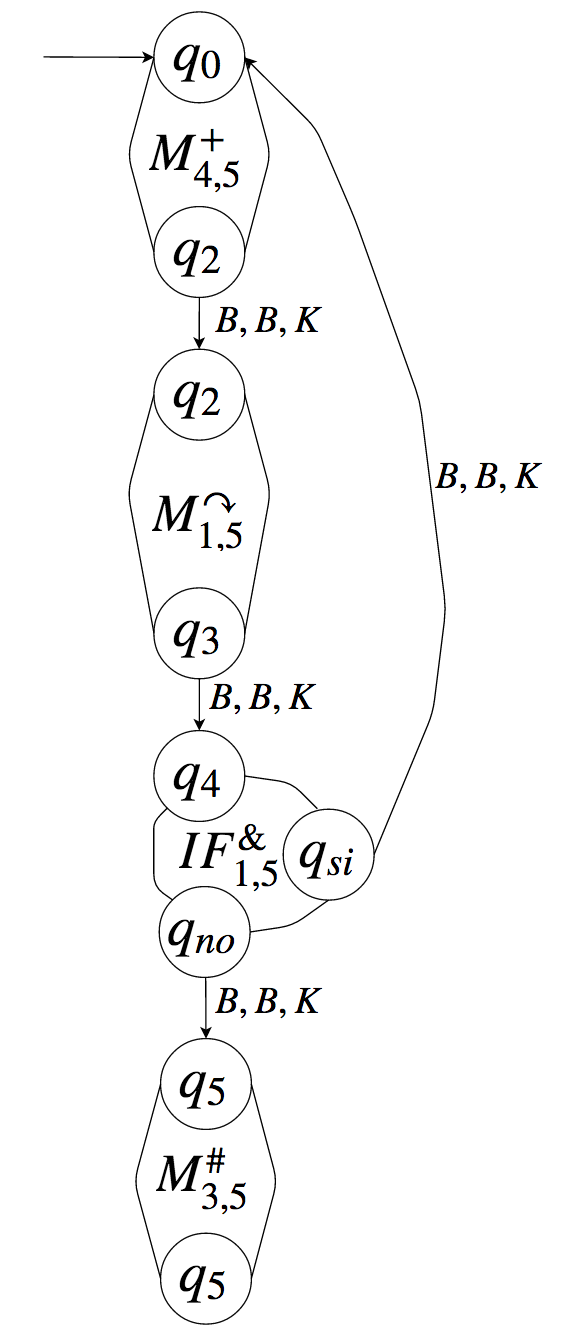
\includegraphics[scale=0.25]{graphics/figure_8.png}
  \end{figure}
\end{frame}

\begin{frame}
  Veamos con un ejemplo como $M_{sim}$ simula a $\mathcal{P}$. Supongamos que
  corremos $\mathcal{P}$ desde el estado%
  \begin{equation*}
  \left\Vert 2,1,0,5,3,\#\&\#\#,\varepsilon ,\&\&,\#\&,\#\right\Vert
  \end{equation*}%
  Tendremos entonces la siguiente sucesion de descripciones instantaneas:%
  \begin{eqnarray*}
  &&(1,\left\Vert 2,1,0,5,3,\#\&\#\#,\varepsilon ,\&\&,\#\&,\#\right\Vert ) \\
  && \\
  &&(2,\left\Vert 2,1,0,6,3,\#\&\#\#,\varepsilon ,\&\&,\#\&,\#\right\Vert ) \\
  && \\
  &&(3,\left\Vert 2,1,0,6,3,\&\#\#,\varepsilon ,\&\&,\#\&,\#\right\Vert ) \\
  && \\
  &&(1,\left\Vert 2,1,0,6,3,\&\#\#,\varepsilon ,\&\&,\#\&,\#\right\Vert ) \\
  && \\
  &&(2,\left\Vert 2,1,0,7,3,\&\#\#,\varepsilon ,\&\&,\#\&,\#\right\Vert ) \\
  && \\
  &&(3,\left\Vert 2,1,0,7,3,\#\#,\varepsilon ,\&\&,\#\&,\#\right\Vert ) \\
  && \\
  &&(4,\left\Vert 2,1,0,7,3,\#\#,\varepsilon ,\&\&,\#\&,\#\right\Vert ) \\
  && \\
  &&(5,\left\Vert 2,1,0,7,3,\#\#,\varepsilon ,\&\&\#,\#\&,\#\right\Vert )
  \end{eqnarray*}

\end{frame}

\begin{frame}
  \begin{figure}[h]
    \centering
    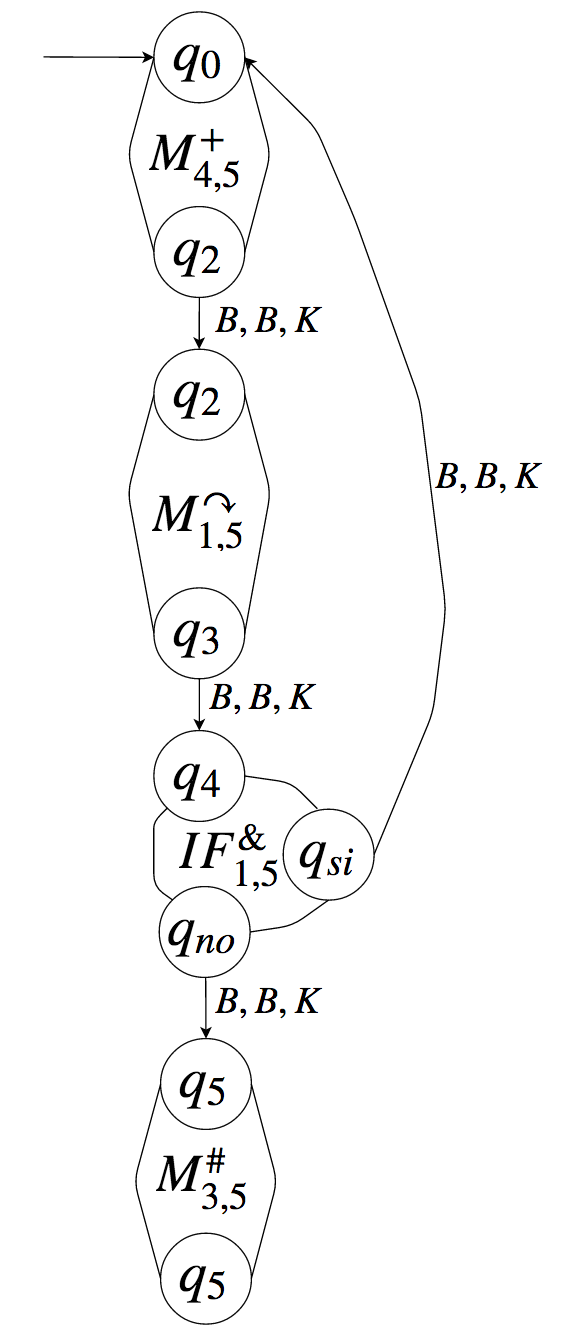
\includegraphics[scale=0.25]{graphics/figure_8.png}
  \end{figure}
\end{frame}

\begin{frame}
  \begin{eqnarray*}
    && q_{1} B \shortmid^{2} B \shortmid BB \shortmid^{7} B \shortmid^{3} B \&\#\# BB \&\& B \#\& B \# B \\
    && q_{2} B \shortmid^{2} B \shortmid BB \shortmid^{7} B \shortmid^{3} B \&\#\# BB \&\& B \#\& B \# B \\
    && \\
    && q_{3} B \shortmid^{2} B \shortmid BB \shortmid^{7} B \shortmid^{3} B \#\# BB \&\& B \#\& B \# B \\
    && q_{4} B \shortmid^{2} B \shortmid BB \shortmid^{7} B \shortmid^{3} B \#\# BB \&\& B \#\& B \# B \\
    && \\
    && q_{no} B \shortmid^{2} B \shortmid BB \shortmid^{7} B \shortmid^{3} B \#\# BB \&\& B \#\& B \# B \\
    && q_{5} B \shortmid^{2} B \shortmid BB \shortmid^{7} B \shortmid^{3} B \#\# BB \&\& B \#\& B \# B \\
    && \\
    && q_{6} B \shortmid^{2} B \shortmid BB \shortmid^{7} B \shortmid^{3} B \#\# BB \&\&\# B \#\& B \# B
  \end{eqnarray*}
\end{frame}

\begin{frame}
  \begin{block}
    \PN Supongamos que $\mathcal{P} = I_{1}, \dotsc, I_{n}$. Para cada $i = 1, \dotsc, n$, llamaremos $M_{i}$ a la
    máquina que simulará el efecto que produce la instrucción $I_{i}$, es decir tomemos:
    \begin{enumerate}
      \item[-] $M_{i}=M_{j,k}^{+}$, si $Bas(I_{i})=\mathrm{N}\bar{j}\leftarrow
      \mathrm{N}\bar{j}+1$

      \item[-] $M_{i}=M_{j,k}^{\dot{-}}$, si $Bas(I_{i})=\mathrm{N}\bar{j}%
      \leftarrow \mathrm{N}\bar{j}\dot{-}1$

      \item[-] $M_{i}=M_{j,k}^{a}$, si $Bas(I_{i})=\mathrm{P}\bar{j}\leftarrow
      \mathrm{P}\bar{j}.a$

      \item[-] $M_{i}=M_{j,k}^{\curvearrowright }$, si $Bas(I_{i})=\mathrm{P}\bar{j%
      }\leftarrow \ ^{\curvearrowright }\mathrm{P}\bar{j}$

      \item[-] $M_{i}=M_{j\leftarrow m}^{\#,k}$, si $Bas(I_{i})=\mathrm{N}\bar{j}%
      \leftarrow \mathrm{N}\bar{m}$

      \item[-] $M_{i}=M_{j\leftarrow m}^{\ast ,k}$, si $Bas(I_{i})=\mathrm{P}\bar{j%
      }\leftarrow \mathrm{P}\bar{m}$

      \item[-] $M_{i}=M_{j\leftarrow 0}^{k}$, si $Bas(I_{i})=\mathrm{N}\bar{j}%
      \leftarrow 0$

      \item[-] $M_{i}=M_{j\leftarrow \varepsilon }^{k}$, si $Bas(I_{i})=\mathrm{P}%
      \bar{j}\leftarrow \varepsilon $

      \item[-] $M_{i}=M_{\mathrm{SKIP}}$, si $Bas(I_{i})=\mathrm{SKIP}$

      \item[-] $M_{i}=IF_{j,k}$, si $Bas(I_{i})=\mathrm{IF}\;\mathrm{N}\bar{j}%
      \not=0$\ $\mathrm{GOTO}\;\mathrm{L}\bar{m}$, para algún $m$

      \item[-] $M_{i}=IF_{j,k}^{a}$, si $Bas(I_{i})=\mathrm{IF}\;\mathrm{P}\bar{j}%
      \;\mathrm{BEGINS}\;a\;\mathrm{GOTO}\;\mathrm{L}\bar{m}$, para algún $m$
    \end{enumerate}
  \end{block}
\end{frame}

\begin{frame}
  \PN Ya que la máquina $M_{i}$ puede tener uno o dos estados finales, la representaremos de la siguiente manera:
  \begin{figure}[h]
    \centering
    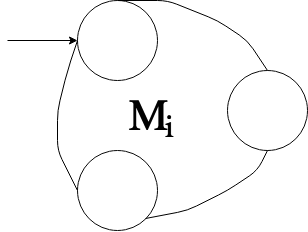
\includegraphics[scale=0.4]{graphics/figure_5.png}
  \end{figure}
  \begin{itemize}
    \item Si $M_{i}$ tiene \textbf{un solo estado final}, este está representado por el círculo de abajo a la izquierda
    \item Si $M_{i}$ tiene \textbf{dos estados finales}, el estado final de la derecha corresponde al estado $q_{si}$ y
      el de la izquierda al estado $q_{no}$.
  \end{itemize}
\end{frame}

\begin{frame}
  \begin{block}
    \PN Supongamos que $\mathcal{P} = I_{1}, \dotsc, I_{n}$. Para cada $i = 1, \dotsc, n$, llamaremos $M_{i}$ a la
    máquina que simulará el efecto que produce la instrucción $I_{i}$, es decir tomemos:
    \begin{enumerate}
      \item[-] $M_{i}=M_{j,k}^{+}$, si $Bas(I_{i}) = \mathrm{N}\bar{j} \leftarrow \mathrm{N}\bar{j}+1$

      \item[-] $M_{i}=M_{j,k}^{\dot{-}}$, si $Bas(I_{i}) = \mathrm{N}\bar{j} \leftarrow \mathrm{N}\bar{j}\dot{-}1$

      \item[-] $M_{i}=M_{j,k}^{a}$, si $Bas(I_{i})=\mathrm{P}\bar{j} \leftarrow \mathrm{P}\bar{j}.a$

      \item[-] $M_{i}=M_{j,k}^{\curvearrowright }$, si $Bas(I_{i}) = \mathrm{P}\bar{j} \leftarrow \
      ^{\curvearrowright}\mathrm{P}\bar{j}$

      \item[-] $M_{i}=M_{j\leftarrow m}^{\#,k}$, si $Bas(I_{i}) = \mathrm{N}\bar{j} \leftarrow \mathrm{N}\bar{m}$

      \item[-] $M_{i}=M_{j\leftarrow m}^{\ast ,k}$, si $Bas(I_{i}) = \mathrm{P}\bar{j} \leftarrow \mathrm{P}\bar{m}$

      \item[-] $M_{i}=M_{j\leftarrow 0}^{k}$, si $Bas(I_{i}) = \mathrm{N}\bar{j} \leftarrow 0$

      \item[-] $M_{i}=M_{j\leftarrow \varepsilon }^{k}$, si $Bas(I_{i}) = \mathrm{P}\bar{j} \leftarrow \varepsilon$

      \item[-] $M_{i}=M_{\mathrm{SKIP}}$, si $Bas(I_{i}) = \mathrm{SKIP}$

      \item[-] $M_{i}=IF_{j,k}$, si $Bas(I_{i})=\mathrm{IF}\;\mathrm{N}\bar{j} \neq 0 \ \mathrm{GOTO}\;
      \mathrm{L}\bar{m}$, para algún $m$

      \item[-] $M_{i}=IF_{j,k}^{a}$, si $Bas(I_{i}) = \mathrm{IF}\;\mathrm{P}\bar{j} \;\mathrm{BEGINS}\;a\;\mathrm{GOTO}
      \;\mathrm{L}\bar{m}$, para algún $m$
    \end{enumerate}
  \end{block}
\end{frame}

\begin{frame}
  \begin{alertblock}{Lema}
    \PN Sea $\mathcal{P} \in \mathrm{Pro}^{\Sigma}$ y sea $k \geq N(\mathcal{P})$. Supongamos que en $\mathcal{P}$ no
    hay instrucciones de la forma $\mathrm{GOTO} \ \mathrm{L}\bar{m}$ ni de la forma $\mathrm{L}\bar{n} \ \mathrm{GOTO}
    \ \mathrm{L}\bar{m}$. Sean:
    \begin{itemize}
      \item Para cada $a \in \Sigma \cup \{\shortmid\}$, sea $\tilde{a}$ un nuevo símbolo
      \item $\Gamma = \Sigma \cup \{B, \shortmid\} \cup \{\tilde{a}: a \in \Sigma \cup \{\shortmid\}\}$
    \end{itemize}
    \PN entonces existe una máquina de Turing determinística con unit $M = \left(Q, \Gamma, \Sigma, \delta, q_{0}, B,
    \shortmid,\{q_{f}\}\right)$, la cual satisface:
    \begin{enumerate}[1)]
      \item $\delta (q_{f},\sigma) = \emptyset$, para cada $\sigma \in \Gamma$.

      \item Cualesquiera sean $x_{1}, \dotsc, x_{k} \in \omega$ y $\alpha_{1}, \dotsc, \alpha_{k} \in \SIGMA$, el
      programa $\mathcal{P}$ se detiene partiendo del estado
      \begin{equation*}
        \lVert x_{1}, \dotsc, x_{k}, \alpha_{1}, \dotsc, \alpha_{k} \rVert
      \end{equation*}
      \PN si y solo si $M$ se detiene partiendo de la descripción instantanea
      \begin{equation*}
        \left\lfloor q_{0} B \shortmid^{x_{1}} B \dotsc B \shortmid^{x_{k}} B \alpha_{1} B \dotsc B \alpha_{k} B
        \right\rfloor
      \end{equation*}
    \end{enumerate}
  \end{alertblock}
\end{frame}

\begin{frame}
  \PN Para armar la máquina que simulará a $\mathcal{P}$ hacemos lo siguiente:
  \begin{enumerate}[1)]
    \item Primero unimos las maquinas $M_{1}, \dotsc, M_{n}$ de la siguiente manera
      \begin{figure}[h]
        \centering
        \includegraphics[scale=0.24]{graphics/figure_6.png}
      \end{figure}
  \end{enumerate}
\end{frame}

\begin{frame}
  \PN $I_{j}$ cumplirá que:
  \begin{equation*}
    \begin{array}{lcr}
      \alpha B \beta_{j} B \dotsc B \beta_{2} B \beta_{1} B \gamma &\overset{\ast}{\vdash}& \alpha B \beta_{j} B \dotsc
        B \beta_{2} B \beta_{1} B \gamma \\
      \ \ \ \ \ \ \ \ \ \ \ \ \ \ \ \ \ \ \ \ \ \ \ \ \ \ \ \ \uparrow && \uparrow \ \ \ \ \ \ \ \ \ \ \ \ \ \ \ \ \ \
        \ \ \ \ \ \ \ \ \ \  \\
      \ \ \ \ \ \ \ \ \ \ \ \ \ \ \ \ \ \ \ \ \ \ \ \ \ \ \ \ \ q_{0} && q_{f} \ \ \ \ \ \ \ \ \ \ \ \ \ \ \ \ \ \ \ \
        \ \ \ \ \ \ \ \
    \end{array}%
  \end{equation*}%
  \PN siempre que $\alpha, \gamma \in \Gamma^{\ast}, \beta_{1}, \dotsc, \beta_{j} \in (\Gamma - \{B\})^{\ast}$. Dejamos
  al lector la manufactura de esta máquina.

  \vspace{3mm}
  \PN Para $j \geq 1$, sea $TD_{j}$ una máquina con un solo estado final $q_{f}$ y tal que:
  \begin{equation*}
    \begin{array}{ccc}
      \alpha B \gamma &\overset{\ast}{\vdash}& \alpha BB \gamma \\
      \uparrow  && \uparrow \ \ \\
      q_{0} &  & q_{f} \ \
    \end{array}
  \end{equation*}
  \PN cada vez que $\alpha, \gamma \in \Gamma^{\ast}$ y $\gamma$ tiene exactamente $j$ ocurrencias de $B$.
\end{frame}

\begin{frame}
  \PN $I_{j}$ cumplirá que:
  \begin{equation*}
    \begin{array}{lcr}
      \alpha B \beta_{j} B \dotsc B \beta_{2} B \beta_{1} B \gamma &\overset{\ast}{\vdash}& \alpha B \beta_{j} B \dotsc
        B \beta_{2} B \beta_{1} B \gamma \\
      \ \ \ \ \ \ \ \ \ \ \ \ \ \ \ \ \ \ \ \ \ \ \ \ \ \ \ \ \uparrow && \uparrow \ \ \ \ \ \ \ \ \ \ \ \ \ \ \ \ \ \
        \ \ \ \ \ \ \ \ \ \  \\
      \ \ \ \ \ \ \ \ \ \ \ \ \ \ \ \ \ \ \ \ \ \ \ \ \ \ \ \ \ q_{0} && q_{f} \ \ \ \ \ \ \ \ \ \ \ \ \ \ \ \ \ \ \ \
        \ \ \ \ \ \ \ \
    \end{array}%
  \end{equation*}%
  \PN siempre que $\alpha, \gamma \in \Gamma^{\ast}, \beta_{1}, \dotsc, \beta_{j} \in (\Gamma - \{B\})^{\ast}$. Dejamos
  al lector la manufactura de esta máquina.

  \vspace{3mm}
  \PN Para $j \geq 1$, sea $TD_{j}$ una máquina con un solo estado final $q_{f}$ y tal que:
  \begin{equation*}
    \begin{array}{ccc}
      \alpha B \gamma &\overset{\ast}{\vdash}& \alpha BB \gamma \\
      \uparrow  && \uparrow \ \ \\
      q_{0} &  & q_{f} \ \
    \end{array}
  \end{equation*}
  \PN cada vez que $\alpha, \gamma \in \Gamma^{\ast}$ y $\gamma$ tiene exactamente $j$ ocurrencias de $B$.
\end{frame}

\begin{frame}
  \begin{alertblock}{}
      \begin{enumerate}[3)]
        \item Si $x_{1}, \dotsc, x_{k} \in \omega$ y $\alpha_{1}, \dotsc, \alpha_{k} \in \SIGMA$ son tales que
        $\mathcal{P}$ se detiene partiendo del estado
        \begin{equation*}
          \lVert x_{1}, \dotsc, x_{k}, \alpha_{1}, \dotsc, \alpha_{k} \rVert
        \end{equation*}
        \PN y llega al estado
        \begin{equation*}
          \lVert y_{1}, \dotsc, y_{k}, \beta_{1}, \dotsc, \beta_{k} \rVert
        \end{equation*}
        \PN entonces

        \sizeOfLetterSecond
        \begin{equation*}
          \left\lfloor q_{0} B \shortmid^{x_{1}} B \dotsc B \shortmid^{x_{k}} B \alpha_{1} B \dotsc B \alpha_{k} B
          \right\rfloor \overset{\ast}{\underset{M}{\vdash}} \left\lfloor q_{f} B \shortmid^{y_{1}} B \dotsc B
          \shortmid^{y_{k}} B \beta_{1} B \dotsc B \beta_{k} B \right\rfloor
        \end{equation*}
      \end{enumerate}
  \end{alertblock}
\end{frame}

\begin{frame}
  \PN Análogamente, para $j \geq 1$, sea $TI_{j}$ una máquina tal que
  \begin{equation*}
    \begin{array}{ccc}
    \alpha B\sigma \gamma  & \overset{\ast }{\vdash } & \alpha B\gamma  \\
    \uparrow \  &  & \uparrow  \\
    q_{0}\ \  &  & q_{f}%
    \end{array}%
  \end{equation*}%
  \PN cada vez que $\alpha \in \Gamma^{\ast}, \sigma \in \Gamma$ y $\gamma$ tiene exactamente $j$ ocurrencias de $B$.
  Dejamos al lector la construcción de, por ejemplo, $TI_{3}$ para $\Sigma = \{\&,\#\}$.

  \vspace{3mm}
  \PN Teniendo las máquinas auxiliares antes definidas podemos combinarlas para obtener las máquinas simuladoras de
  instrucciones.
\end{frame}

\begin{frame}
  \PN $I_{j}$ cumplirá que:
  \begin{equation*}
    \begin{array}{lcr}
      \alpha B \beta_{j} B \dotsc B \beta_{2} B \beta_{1} B \gamma &\overset{\ast}{\vdash}& \alpha B \beta_{j} B \dotsc
        B \beta_{2} B \beta_{1} B \gamma \\
      \ \ \ \ \ \ \ \ \ \ \ \ \ \ \ \ \ \ \ \ \ \ \ \;\; \uparrow && \uparrow \ \ \ \ \ \ \ \ \ \ \ \ \ \ \ \ \ \ \ \ \
        \ \ \  \\
      \ \ \ \ \ \ \ \ \ \ \ \ \ \ \ \ \ \ \ \ \ \ \ \ q_{0} && q_{f} \ \ \ \ \ \ \ \ \ \ \ \ \ \ \ \ \ \ \ \ \ \ \
    \end{array}
  \end{equation*}
  \PN siempre que $\alpha, \gamma \in \Gamma^{\ast}, \beta_{1}, \dotsc, \beta_{j} \in (\Gamma - \{B\})^{\ast}$. Dejamos
  al lector la manufactura de esta máquina.

  \vspace{3mm}
  \PN Para $j \geq 1$, sea $TD_{j}$ una máquina con un solo estado final $q_{f}$ y tal que:
  \begin{equation*}
    \begin{array}{ccc}
      \alpha B \gamma &\overset{\ast}{\vdash}& \alpha BB \gamma \\
      \uparrow  && \uparrow \ \ \\
      q_{0} &  & q_{f} \ \
    \end{array}
  \end{equation*}
  \PN cada vez que $\alpha, \gamma \in \Gamma^{\ast}$ y $\gamma$ tiene exactamente $j$ ocurrencias de $B$.
\end{frame}

\begin{frame}
  \PN \underline{\textbf{Ejemplo:}} Sea $\Sigma = \{a\}$ podemos tomar $TD_{3}$ igual a la siguiente máquina
  \begin{figure}[h]
    \centering
    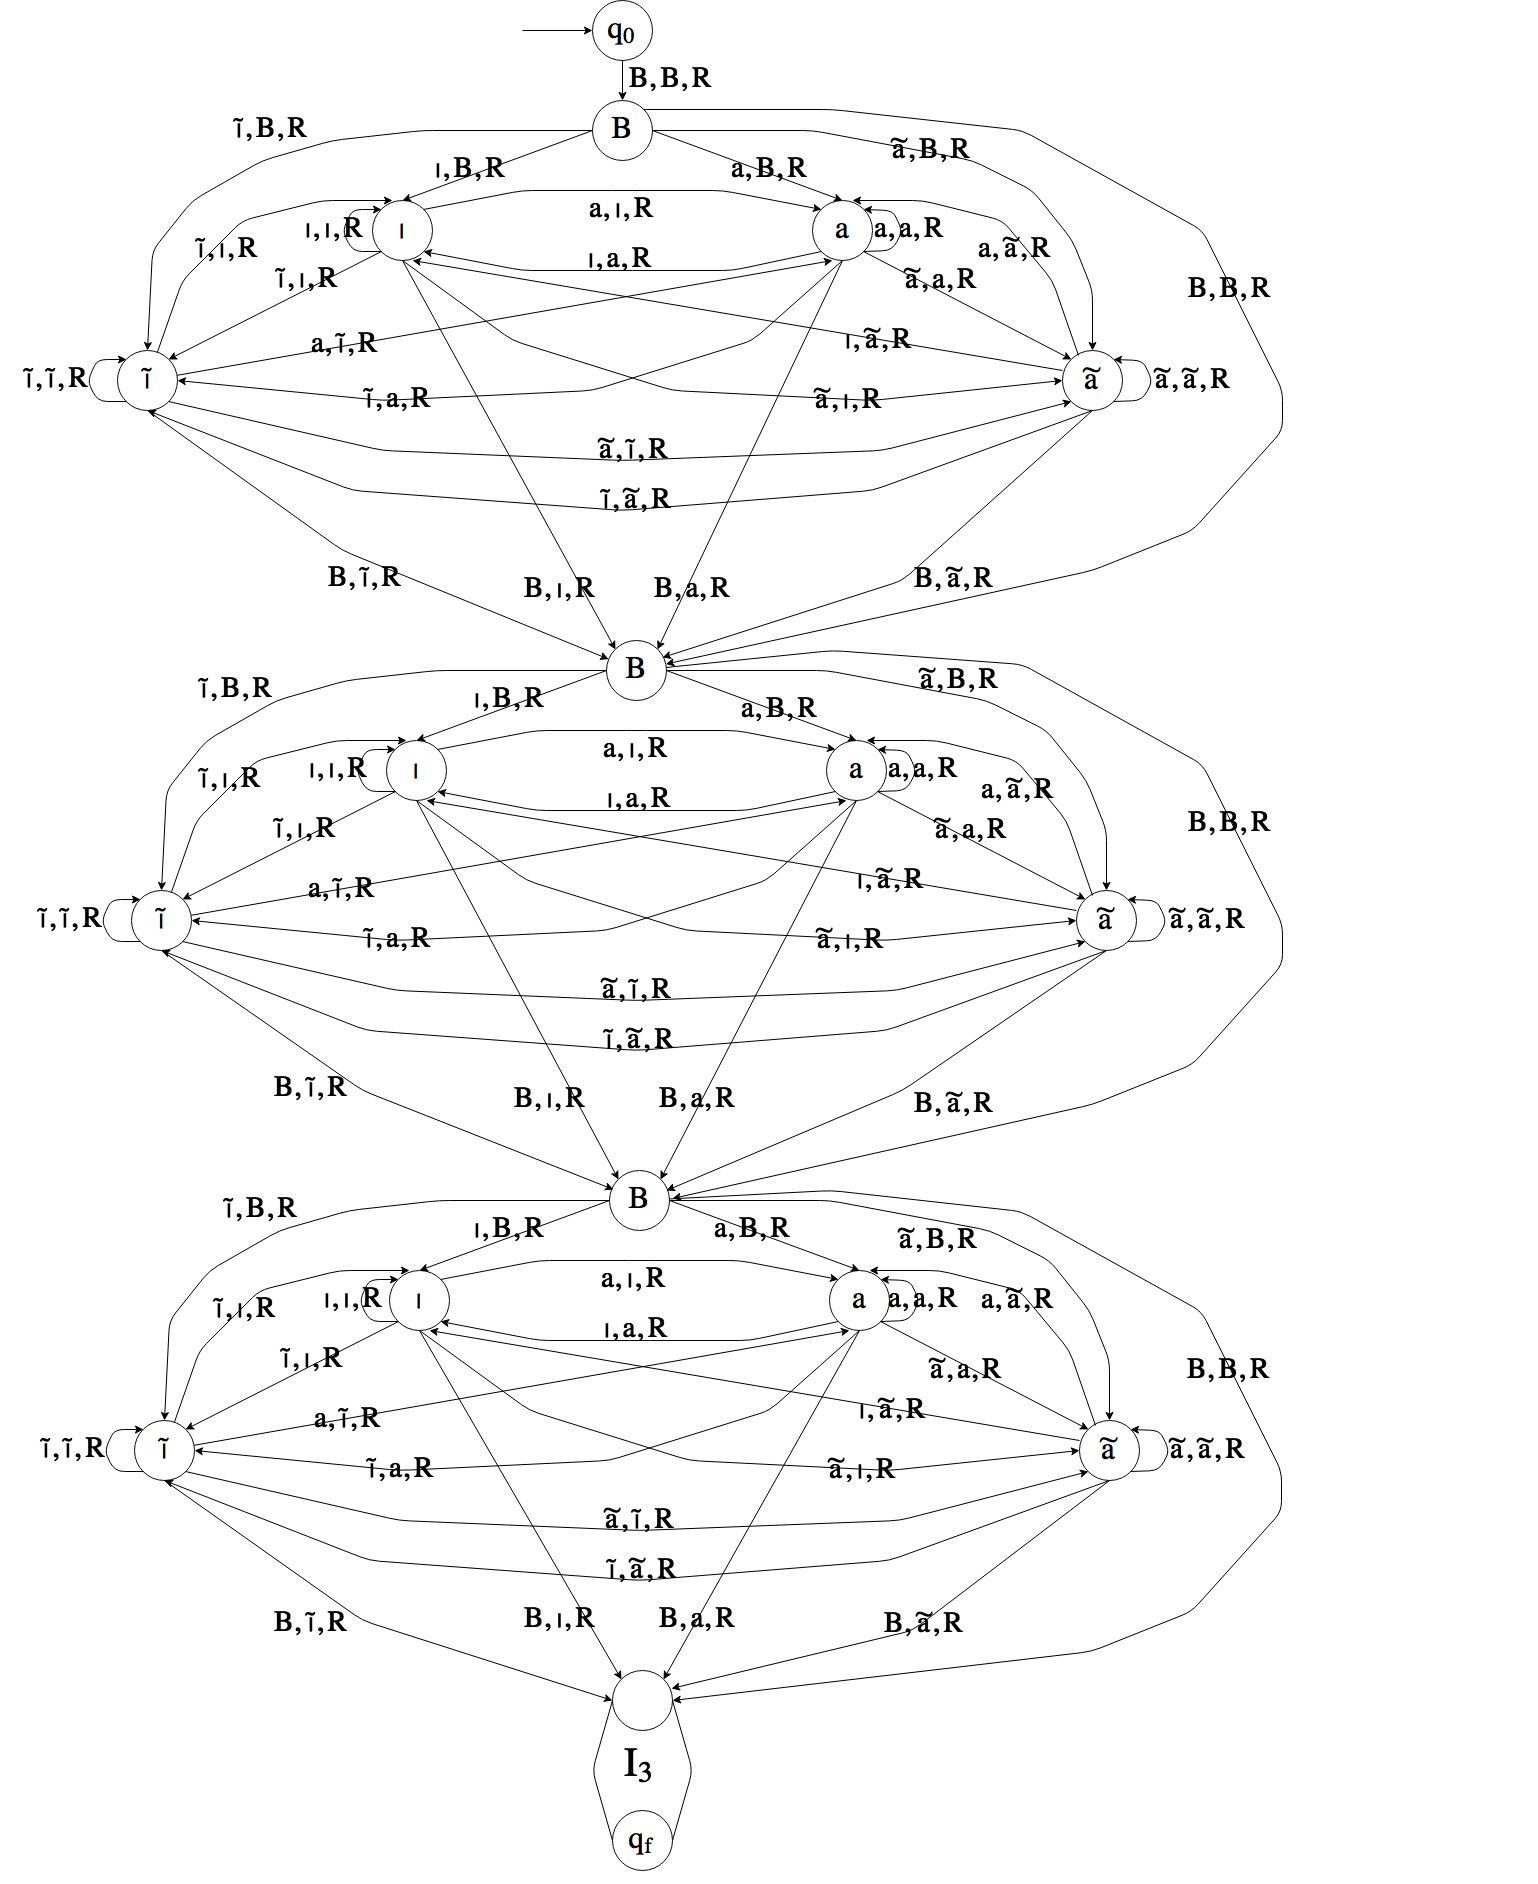
\includegraphics[scale=0.125]{graphics/figure_3.png}
  \end{figure}
\end{frame}

\begin{frame}
  \PN Análogamente, para $j \geq 1$, sea $TI_{j}$ una máquina tal que
  \begin{equation*}
    \begin{array}{ccc}
    \alpha B \sigma \gamma &\overset{\ast}{\vdash}& \alpha B \gamma \\
    \uparrow \ && \uparrow \\
    q_{0} \ \ && q_{f}
    \end{array}
  \end{equation*}
  \PN cada vez que $\alpha \in \Gamma^{\ast}, \sigma \in \Gamma$ y $\gamma$ tiene exactamente $j$ ocurrencias de $B$.
  Dejamos al lector la construcción de, por ejemplo, $TI_{3}$ para $\Sigma = \{\&,\#\}$.

  \vspace{7mm}
  \begin{alertblock}
  \PN Teniendo las máquinas auxiliares antes definidas podemos combinarlas para obtener las máquinas simuladoras de
  instrucciones.
\end{alertblock}
\end{frame}

\begin{frame}

  En lo que sigue probaremos que el paradigma computacional de Turing
es por lo menos tan expresivo como el paradigma imperativo dado por el
lenguaje $\mathcal{S}^{\Sigma }$, es decir probaremos que toda funcion $%
\Sigma $-computable es $\Sigma $-Turing computable\textit{.} Antes un lema

\bigskip

\begin{lemma}
\label{sinGOTO}Si $f:D_{f}\subseteq \omega ^{n}\times \Sigma ^{\ast
m}\rightarrow \Sigma ^{\ast }$ es $\Sigma $-computable, entonces hay un
programa $\mathcal{Q}$ el cual computa a $f$ y el cual cumple con las
siguientes propiedades

\begin{enumerate}
\item[(1)] En $\mathcal{Q}$ no hay instrucciones de la forma $\mathrm{GOTO}\;%
\mathrm{L}\bar{\imath}$ ni de la forma $\mathrm{L}\bar{j}\ \mathrm{GOTO}\;%
\mathrm{L}\bar{\imath}$

\item[(2)] Cuando $\mathcal{Q}$ termina partiendo de un estado cualquiera
dado, el estado alcansado es tal que las variables numericas tienen todas el
valor $0$ y las alfabeticas tienen todas exepto $\mathrm{P}1$ el valor $%
\varepsilon $.
\end{enumerate}
\end{lemma}

\end{frame}

\begin{frame}
  \begin{proof}
    \PN Sean:
    \begin{itemize}
      \item $\mathcal{P}$ un programa que compute a $f$
      \item $r \in \mathbf{N}$ tal que $r \geq N(\mathcal{P}), n, m$
      \item $\mathcal{\tilde{P}}$ el resultado de reemplazar en $\mathcal{P}$ cada instrucción de la forma $\alpha
      \mathrm{GOTO} \ \mathrm{L}\bar{\imath}$ con $\alpha \in \{\varepsilon\} \cup \{\mathrm{L}\bar{j}: j \in
      \mathbf{N}\}$ por $\alpha \mathrm{IF \ N}\bar{r} \neq 0 \ \mathrm{GOTO} \ \mathrm{L}\bar{\imath}$.
    \end{itemize}

    \PN Ahora, sea $\mathcal{Q}$ el siguiente programa:
    \begin{equation*}
      \begin{array}{l}
        \mathrm{N}\bar{r} \leftarrow \mathrm{N}\bar{r} + 1 \\
        \mathcal{\tilde{P}} \\
        \mathrm{N}1\leftarrow 0 \\
        \vdots \\
        \mathrm{N}\bar{r} \leftarrow 0 \\
        \mathrm{P}2 \leftarrow \varepsilon  \\
        \vdots \\
        \mathrm{P}\bar{r} \leftarrow \varepsilon
      \end{array}
    \end{equation*}
  \end{proof}
\end{frame}

\begin{frame}

Por supuesto, hay un lema analogo para el caso en que $f$ llega a $\omega $
en lugar de llegar a $\Sigma ^{\ast }$

\bigskip

Ahora si, el anunciado del teorema:

\begin{theorem}
Si $f:D_{f}\subseteq \omega ^{n}\times \Sigma ^{\ast m}\rightarrow O$ es $%
\Sigma $-computable, entonces $f$ es $\Sigma $-Turing computable\textit{.}
\end{theorem}
\end{frame}

\begin{frame}
  \begin{proof}
  Supongamos $O=\Sigma ^{\ast }$. Por el Lema \ref{sinGOTO} existe $\mathcal{P}%
  \in \mathrm{Pro}^{\Sigma }$ el cual computa $f$ y tiene las propiedades (1)
  y (2). Sea $k=\max \{n,m,N(\mathcal{P})\}$ y sea $M_{sim}$ la maquina de
  Turing con unit que simula a $\mathcal{P}$ respecto de $k$. Como puede
  observarse, la maquina $M_{sim}$, no necesariamente computara a $f$. Sea $%
  M_{1}$ la maquina siguiente

  Figura 9

  (Cuando $n=0$ debemos interpretar que $D_{0}=\left( \{q_{0},q_{f}\},\Gamma
  ,\Sigma ,\delta ,q_{0},B,\shortmid ,\{q_{f}\}\right) $, con $\delta
  (q_{0},B)=\{(q_{f},B,K)\}$ y $\delta =\emptyset $ en cualquier otro caso).

  Notese que $M_{1}$ cumple que para cada $(\vec{x},\vec{\alpha})\in \omega
  ^{n}\times \Sigma ^{\ast m}$,%
  \begin{equation*}
  \left\lfloor q_{0}B\shortmid ^{x_{1}}B...B\shortmid ^{x_{n}}B\alpha
  _{1}B...B\alpha _{m}B\right\rfloor \overset{\ast }{\vdash }\left\lfloor
  q_{f}B\shortmid ^{x_{1}}B...B\shortmid ^{x_{n}}B^{k-n}B\alpha
  _{1}B...B\alpha _{m}B\right\rfloor
  \end{equation*}%
  Notese que en la confeccion de $M_{1}$, para el caso $m>0$ podriamos haber
  usado directamente la $TD_{m}$ en lugar de usar $TD_{m}$.

  Sea $M_{2}$ la siguiente maquina

  Figura 10

  Notese que $M_{2}$ cumple que para cada $\alpha \in \Sigma ^{\ast }$,%
  \begin{equation*}
  \left\lfloor q_{0}B^{k+1}\alpha \right\rfloor \overset{\ast }{\vdash }%
  \left\lfloor q_{f}B\alpha \right\rfloor
  \end{equation*}%
  Sea $M$ la maquina dada por el siguiente diagrama

  Figura 11

  A continuacion veremos que $M$ computa a $f$. Supongamos que $(\vec{x},\vec{%
  \alpha})\in (\omega ^{n}\times \Sigma ^{\ast m})-D_{f}$. Deberemos ver que $M
  $ no termina partiendo de

  \begin{enumerate}
  \item[(*)] $\left\lfloor q_{0}B\shortmid ^{x_{1}}B...B\shortmid
  ^{x_{n}}B\alpha _{1}B...B\alpha _{m}B\right\rfloor $
  \end{enumerate}

  Primero notemos que, ya que $\mathcal{P}$ computa a $f$, tenemos que $%
  \mathcal{P}$ no termina partiendo de $\left\Vert x_{1},...,x_{n},\alpha
  _{1},...,\alpha _{m}\right\Vert $ por lo cual $\mathcal{P}$ no termina
  partiendo de%
  \begin{equation*}
  \left\Vert x_{1},...,x_{n},\overset{k-n}{\overbrace{0,...,0}},\alpha
  _{1},...,\alpha _{m},\overset{k-m}{\overbrace{\varepsilon ,...,\varepsilon }}%
  \right\Vert
  \end{equation*}%
  lo cual implica (Lema \ref{simulacion}) que

  \begin{enumerate}
  \item[(**)] $M_{sim}$ no termina partiendo de $\left\lfloor q_{0}B\shortmid
  ^{x_{1}}B...B\shortmid ^{x_{n}}B^{k-n}B\alpha _{1}B...B\alpha
  _{m}B\right\rfloor $
  \end{enumerate}

  Ahora notese que si hacemos funcionar a $M$ desde la descripcion instantanea
  dada en (*), llegaremos (via la copia de $M_{1}$ dentro de $M$)
  indefectiblemente (ya que $M$ es deterministica) a la siguiente descripcion
  instantanea%
  \begin{equation*}
  \left\lfloor q_{2}B\shortmid ^{x_{1}}B...B\shortmid ^{x_{n}}B^{k-n}B\alpha
  _{1}B...B\alpha _{m}B\right\rfloor
  \end{equation*}%
  Luego entonces (**) nos dice que al seguir trabajando $M$ (ahora via la
  copia de $M_{sim}$ dentro de $M$), la maquina $M$ nunca terminara.

  Para terminar de ver que $M$ computa a $f$, tomemos $(\vec{x},\vec{\alpha}%
  )\in D_{f}$ y veamos que%
  \begin{equation*}
  \left\lfloor q_{0}B\shortmid ^{x_{1}}B...B\shortmid ^{x_{n}}B\alpha
  _{1}B...B\alpha _{m}B\right\rfloor \overset{\ast }{\underset{M}{\vdash }}%
  \left\lfloor q_{5}Bf(\vec{x},\vec{\alpha})\right\rfloor
  \end{equation*}%
  y que la maquina $M$ se detiene en $\left\lfloor q_{5}Bf(\vec{x},\vec{\alpha}%
  )\right\rfloor $. La maquina $M$ se detiene en $\left\lfloor q_{5}Bf(\vec{x},%
  \vec{\alpha})\right\rfloor $ ya que $q_{5}$ es el estado final de una copia
  de $M_{2}$ y por lo tanto no sale ninguna flecha desde el. Ya que $\mathcal{P%
  }$ computa a $f$ y tiene la propiedad (2) del Lema \ref{sinGOTO}, tenemos
  que $\mathcal{P}$ termina partiendo de $\left\Vert x_{1},...,x_{n},\alpha
  _{1},...,\alpha _{m}\right\Vert $ y llega al estado $\left\Vert f(\vec{x},%
  \vec{\alpha})\right\Vert $, o lo que es lo mismo, $\mathcal{P}$ termina
  partiendo de%
  \begin{equation*}
  \left\Vert x_{1},...,x_{n},\overset{k-n}{\overbrace{0,...,0}},\alpha
  _{1},...,\alpha _{m},\overset{k-m}{\overbrace{\varepsilon ,...,\varepsilon }}%
  \right\Vert
  \end{equation*}%
  y llega al estado%
  \begin{equation*}
  \left\Vert \overset{k}{\overbrace{0,...,0}},f(\vec{x},\vec{\alpha}),\overset{%
  k-1}{\overbrace{\varepsilon ,...,\varepsilon }}\right\Vert
  \end{equation*}%
  Pero entonces el Lema \ref{simulacion} nos dice que

  \begin{enumerate}
  \item[(***)] $\left\lfloor q_{0}B\shortmid ^{x_{1}}B...B\shortmid
  ^{x_{n}}B^{k-n}B\alpha _{1}B...B\alpha _{m}B\right\rfloor \overset{\ast }{%
  \underset{M_{sim}}{\vdash }}\left\lfloor q_{f}B^{k+1}f(\vec{x},\vec{\alpha}%
  )\right\rfloor $
  \end{enumerate}

  Como ya lo vimos, si hacemos funcionar a $M$ desde $\left\lfloor
  q_{0}B\shortmid ^{x_{1}}B...B\shortmid ^{x_{n}}B\alpha _{1}B...B\alpha
  _{m}B\right\rfloor $, llegaremos (via la copia de $M_{1}$ dentro de $M$)
  indefectiblemente a la siguiente descripcion instantanea%
  \begin{equation*}
  \left\lfloor q_{2}B\shortmid ^{x_{1}}B...B\shortmid ^{x_{n}}B^{k-n}B\alpha
  _{1}B...B\alpha _{m}B\right\rfloor
  \end{equation*}%
  Luego (***) nos dice que, via la copia de $M_{sim}$ dentro de $M$,
  llegaremos a $\left\lfloor q_{3}B^{k+1}f(\vec{x},\vec{\alpha})\right\rfloor $
  e inmediatamente a $\left\lfloor q_{4}B^{k+1}f(\vec{x},\vec{\alpha}%
  )\right\rfloor $. Finalmente, via la copia de $M_{2}$ dentro de $M$,
  llegaremos a $\left\lfloor q_{5}Bf(\vec{x},\vec{\alpha})\right\rfloor $, lo
  cual termina de demostrar que $M$ computa a $f$
  \end{proof}
\end{frame}


\end{document}
